\section{Contraction and the continuous calculation}\label{sec:contraction}
The contraction calculation starts from a fully convective model at
$\Teff=2864$ K and $R=1.594\Rs$. Initial deuterium burns first and is
exhausted; proton--proton burning then rises to supply the surface
luminosity (Figure~\ref{fig:pms}). At 1 Gyr the model has $\Teff=2765$ K,
$R=0.1264\Rs$, $L=8.416\times10^{-4}\Ls$, central temperature 4.623 MK and
$\log g=5.234$, with nuclear burning supplying 99.17\% of the light. The
abundances are still uniform, $X=0.6998$ and $X_3=2.402\times10^{-4}$.
The sequence to 1 Gyr contains 1019 accepted intervals and no rejected ones,
and every interval passes the step-doubling, isotope, mass-defect and
first-law checks. Continued with the same settings, the star reaches 4 Gyr
with sustained hydrogen burning; allowing steps up to 1 Gyr on the quiet
main sequence changes the endpoint temperature by $6.936\times10^{-5}$ K.

\begin{figure}[H]\centering
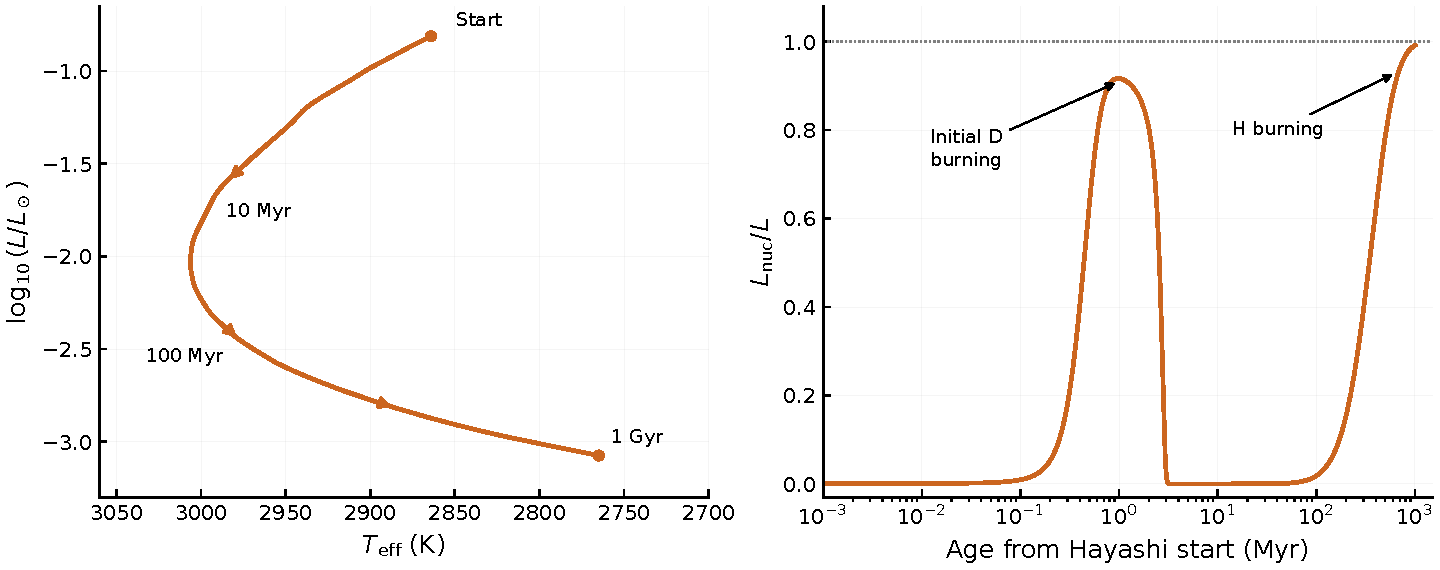
\includegraphics[width=0.92\textwidth]{pms_main_sequence.pdf}
\caption{Contraction of the $0.1\Ms$ model into the main sequence,
computed with the continuous driver. Left: the HR track, arrows showing
increasing age. Right: the fraction of the surface luminosity supplied by
nuclear burning; the early maximum is deuterium burning. Age is measured
from the contracting starting model. The plotted sequence ends at 1 Gyr;
the same calculation continues to 4 Gyr and, with the composition-dependent
atmosphere, to $2.102\Tyr$ (text). It is not joined to Tracks S, F and P.}
\label{fig:pms}
\end{figure}

During deuterium burning the convective travel time is 0.9535--1.415 yr
against local burning times of at least 1949 yr, and the heat carried by
composition redistribution is at most 0.003463\% of the local luminosity;
including ten times that heat produces no resolved change. After deuterium
exhaustion, generous estimates of neutral and Coulomb mobilities give a
microscopic-to-convective diffusion ratio below $6.581\times10^{-9}$, and
ten times the estimated kinetic heat changes the 1 Gyr endpoint by less than
$10^{-3}$ K. These estimates justify whole-star instantaneous mixing while
the star is fully convective; they are not a transport law for partially
ionized gas, and the approximation ends when a radiative region forms.

\paragraph{Comparison with observed stars.}
Table~\ref{tab:observed} compares the continuous model at 1 Gyr with
three measured objects \cite{davis24,agol21,ribas17}. The closest comparison
is the eclipsing companion EBLM J2114$-$39 B, whose mass agrees with
$0.1\Ms$ and whose radius is 1.1\% smaller than Ember's, within its
uncertainty; its metallicity, $[\mathrm{Fe/H}]=-0.001\pm0.032$, matches the
adopted composition. TRAPPIST-1 and Proxima bracket Ember in radius,
temperature and luminosity, but their masses rest on a mass--luminosity
relation and on stellar models respectively. Ten billion years of hydrogen
burning changes Ember's luminosity by less than 0.4\% and its temperature
by less than 2 K, so main-sequence age does not affect the comparison.
The agreement supports the starting structure without establishing
percent-level accuracy or selecting among atmosphere and interior choices.

\begin{table}[H]\centering\small
\caption{Continuous model at 1 Gyr and observed low-mass stars.}\label{tab:observed}
\begin{tabular}{@{}lrrrr@{}}\toprule
Star & Mass ($\Ms$) & Radius ($\Rs$) & $\Teff$ (K) & Luminosity ($\Ls$) \\\midrule
Ember, 1 Gyr & 0.1 & 0.1264 & 2765 & 0.0008416 \\
EBLM J2114$-$39 B & $0.0993\pm0.0033$ & $0.1250\pm0.0016$ & --- & --- \\
TRAPPIST-1 & $0.0898\pm0.0023$ & $0.1192\pm0.0013$ & $2566\pm26$ & $0.000553\pm0.000019$ \\
Proxima & $0.120\pm0.003$ & $0.146\pm0.007$ & $2980\pm80$ & $0.00151\pm0.00008$ \\\bottomrule
\end{tabular}
\end{table}

\paragraph{Continuous hydrogen burning.}
The same program follows contraction, deuterium burning and the main
sequence using composition-dependent atmosphere tables at fixed $Z=0.02$.
A completed calculation reaches $2.102\Tyr$ in 5931 accepted intervals,
66.16 CPU minutes and 35.41 minutes of elapsed time. At that age the star
is still fully mixed, with $X=0.4170$, $\Teff=3020$ K,
$R=0.1485\Rs$, $L=0.001653\Ls$ and central temperature 5.921 MK.
Every accepted interval passes the isotope and energy audits. The
fixed-metal allowance of $10^{-8}$ ultimately rejects 28 trial intervals;
the final, repeatedly halved trial fails the separate energy audit. This
limit belongs to the chosen atmosphere approximation, rather than to an
instability in the accepted stellar structures.

With hot screened transport selected and a fixed-metal allowance of
$2\times10^{-5}$, the continuous model has passed $3.02\Tyr$ with no
rejected intervals. It remains fully convective. A calculation that includes
the restored hydrogen- and metal-dependent atmospheres starts from the same
Hayashi prescription; its initial contraction and relocated restart pass the
same audits. The material selection covers the saved settling structures
through $X=0.9995$ and $Z=10^{-6}$; the trace-helium and white-dwarf
extensions are still needed. Neither continuous calculation has yet reached
the loss of full convection. Tracks S, F and P therefore provide the
late hydrogen-burning comparisons in Section~\ref{sec:hydrogen}.
